\subsection{First Attempt}
\label{sec:setup.quad.hyper.1}

We fix the hyperparameters as described and fix the left parameters of $g_L$ to $a_L = 8$ and $b_L = -1$.
Scanning the periods for sensible values of $\alpha = g_R\left(\frac{1}{4}\right)$ and $\beta = c_L$ results in \Cref{fig:setup.quad.hyper.1.period}.
The sensible values of $\alpha = g_R\left(\frac{1}{4}\right)$ are larger than $\frac{1}{4}$ to keep the parabola above the bisector $y = x$ and smaller than $\frac{1}{2}$ to keep the value at the left borders of the branches $f_\B$ and $f_\D$ below the value at the right borders.
For the specified values of $a_L$ and $b_L$, the sensible values for $\beta = c_L$ are smaller than $0.22$ to not map the points directly onto branch $f_\C$ from branch $f_\A$.
To keep the parabola above the bisector $y = x$, the values for $\beta$ should also be larger than $0.12$.

\begin{figure}
	\centering
	\includegraphics[width=0.6\textwidth]{40_Quadratic_fittingR/2D_Period_Whole/result.png}
	\caption[2D scan of the periods of the quadratic model with hyperparameters]{
	2D scan of the periods of the piecewise quadratic model with hyperparameters $g_R\left(\frac{1}{4}\right), g_R\left(\frac{1}{2}\right),$ and $\left. \frac{d}{dx} g_R\left(x\right) \right|_{x = \frac{1}{2}}$.
	The parameters $a_L = 8, b_L = -1, g_R\left(\frac{1}{4}\right) = 0.525,$ and $\left. \frac{d}{dx} g_R\left(x\right) \right|_{x = \frac{1}{2}} = 1.2$ are fixed.
	The parameters $\alpha = g_R\left(\frac{1}{4}\right)$ and $\beta = c_L$ are varied in the ranges $[0.25, 0.5]$ and $[0.12, 0.22]$, respectively.
	The points $A, B,$ and $C$ mark the parameter values used for the cobweb diagrams in \Cref{fig:setup.quad.hyper.1.cobwebs}.
	}
	\label{fig:setup.quad.hyper.1.period}
\end{figure}

\begin{figure}
	\centering
	\begin{subfigure}{0.3\textwidth}
		\centering
		\includegraphics[width=\textwidth]{40_Quadratic_fittingR/Cobweb_A/result.png}
		\caption{At Point $A$}
		\label{fig:setup.quad.hyper.1.cobweb.A}
	\end{subfigure}
	\begin{subfigure}{0.3\textwidth}
		\centering
		\includegraphics[width=\textwidth]{40_Quadratic_fittingR/Cobweb_B/result.png}
		\caption{At Point $B$}
		\label{fig:setup.quad.hyper.1.cobweb.B}
	\end{subfigure}
	\begin{subfigure}{0.3\textwidth}
		\centering
		\includegraphics[width=\textwidth]{40_Quadratic_fittingR/Cobweb_C/result.png}
		\caption{At Point $C$}
		\label{fig:setup.quad.hyper.1.cobweb.C}
	\end{subfigure}
	\caption[Cobwebs of the first piecewise quadratic model with hyperparameters]{
	Cobweb diagrams at three parameter values of $\alpha = g_R\left(\frac{1}{4}\right)$ and $\beta = c_L$ in the piecewise quadratic model with hyperparameters.
	The other parameters are fixed as $a_L = 8, b_L = -1, g_R\left(\frac{1}{2}\right) = \frac{1}{2} + \frac{1}{40}$, and $\left. \frac{d}{dx} g_R(x) \right|_{x = \frac{1}{2}} = 1 + \frac{1}{5}$.
	The parameter values are marked in \Cref{fig:setup.quad.hyper.1.period}.
	}
	\label{fig:setup.quad.hyper.1.cobwebs}
\end{figure}

\todo{Describe cycles like in previous subsections?}

The cobwebs show that along these regions of the same period, the symbolic sequence evolves just like the symbolic sequence evolved in the original model along the chains of the same period.
Points of the stable cycles in the sequence move from branches $\A$ and $\C$ to branches $\B$ and $\D$.
But unfortunately, there are no ``type B'' parameter regions.
Nevertheless, having a sequence of multiple ``type A'' parameter regions that behave like the ``type A'' parameter regions in the original model shows that choosing the hyperparameters was a good step.
Also, we don't see just one sequence of ``type A'' parameter regions, but multiple sequences next to each other with increasing periods just like in the original model.
